\documentclass{ieeeaccess}
\usepackage[T1]{fontenc}
\usepackage[utf8]{inputenc}
\usepackage{courier}
\makeatletter
\def\ttfamily{\fontfamily{pcr}\fontseries{m}\selectfont}
\makeatother
\usepackage{cite}
\usepackage{amsmath,amssymb,amsfonts}
\usepackage{graphicx}
\graphicspath{{./}}
\usepackage{textcomp}
\usepackage{tabularx}
\usepackage{booktabs}
\usepackage{url}
\usepackage{array}
\usepackage{bm}
\usepackage[hidelinks,bookmarks=false]{hyperref}

\vol{14}
\year{2026}

\def\BibTeX{{\rm B\kern-.05em{\sc i\kern-.025em b}\kern-.08em
    T\kern-.1667em\lower.7ex\hbox{E}\kern-.125emX}}

\begin{document}

% Include title, author, and related information
\title{Retrieval Augmented SLMs versus LLMs for Medical Question Answering: An Energy Infrastructure Economy Evaluation}

\author{\uppercase{Sifat Ali}, \uppercase{Siddartho Sarker Bipro}, \uppercase{Tasmim Rhaman Medha}, \uppercase{Umme Salma Habiba}, \uppercase{Fahim Montasir}}

\address{Department of Computer Science \& Engineering, United International University, Dhaka, Bangladesh}



\markboth
{Sifat Ali \MakeLowercase{\textit{et al.}}: Retrieval-Augmented SLMs versus LLMs for Medical Question Answering}
{Sifat Ali \MakeLowercase{\textit{et al.}}: Retrieval-Augmented SLMs versus LLMs for Medical Question Answering}

\corresp{Corresponding author: Dr. Md. Motaharul Islam}



% Include abstract
\begin{abstract}
    This study evaluates retrieval augmented generation (RAG) for medical question answering (MQA) by comparing a small language model (SLM), a large language model (LLM), and a rule based hybrid routing strategy using a 115 document biomedical corpus and open MQA benchmarks 9,090 predictions per configuration. Primary answer quality evidence comes from these open benchmarks MedQA, MMLU-Med, and PubMedQA, where RAG effects were task-dependent: MMLU Med performance improved for the LLM, while MedQA and PubMedQA label accuracy did not consistently increase with RAG. To assess deployment feasibility, we introduce an Energy Infrastructure Economy (EIE) framework that reports model quality alongside energy, carbon, and infrastructure costs. NVIDIA Management Library (NVML) based measurements on NVIDIA T4 GPUs indicate that SLM+RAG consumed approximately 2.15$\times$ less energy and produced 2.14$\times$ lower CO$_2$e emissions per million queries compared to LLM+RAG 19.82 vs.\ 42.47\,kg CO$_2$e. Automated faithfulness scores $\approx$47--48\% indicated only partial evidence support, highlighting the need for retrieval refinement and claim verifier benchmarking. Within the evaluated corpus, models, and benchmark scope, these findings suggest that retrieval augmented SLMs can deliver comparable automated faithfulness under the tested configuration, with substantially lower deployment cost and environmental impact than LLM+RAG. Clinical validation by practicing physicians is planned as follow up work; this manuscript does not present real world clinical safety or effectiveness results.
\end{abstract}


% Include keywords
\begin{keywords}
    Green AI, Retrieval Augmented Generation, Small Language Models, Medical Question Answering, Energy Efficiency, Sustainability Metrics
\end{keywords}
    

\titlepgskip=-15pt

\maketitle

\section{Introduction}
\label{sec:introduction}
LLMs have demonstrated strong capabilities in medical question answering (MQA) and related clinical NLP tasks, achieving competitive performance across a variety of benchmark settings~\cite{singhal2025toward}. Realizing this potential in practice, however, requires balancing answer quality with computational efficiency~\cite{singhal2025toward}. Although LLMs can generate high quality responses, they typically demand substantial computational resources, including high-capacity GPUs, memory footprints exceeding 14\,GB, and considerable energy consumption. These requirements restrict deployment in healthcare environments with limited computational infrastructure, such as rural clinics, edge devices, and resource constrained hospitals.

SLMs offer an alternative by operating with fewer parameters and lower computational demands~\cite{xiong2024rag,amugongo2025retrieval}.
 Their reduced resource requirements enable local deployment and improved accessibility, but they often produce shorter or less comprehensive responses, which may limit clinical usefulness. This raises an important research question: can retrieval augmented SLMs narrow the efficiency quality gap relative to LLMs for \emph{benchmark} medical question answering, without claiming validation for clinical deployment?

Sustainability considerations further motivate this investigation~\cite{ren2024reconciling,dauner2025ai}. The energy consumption and carbon emissions associated with model inference generally increase with model size and query volume, making operational efficiency an increasingly important dimension of healthcare AI evaluation. Recent work has accordingly called for reporting resource utilization, energy consumption, and environmental impact alongside traditional clinical performance metrics~\cite{yang2025rag}.

Despite these advances, several important challenges remain. First, RAG does not consistently improve answer quality across medical domains, datasets, and evaluation benchmarks~\cite{yang2025rag}. Second, complexity based routing strategies must balance classification accuracy against latency and computational overhead. Third, ensuring safety and clinical validity requires rigorous clinician evaluation and regulatory assessment prior to real world deployment~\cite{labkoff2024aicds,tam2024quest}. Finally, evidence grounding and faithfulness mitigation remain open challenges that call for explicit baselines and systematic evaluation~\cite{asgari2022hallucination,nishizaki2025reducing}.

\subsection{Research Questions}

Motivated by these challenges, this study addresses the following research questions:

\textbf{RQ1:} Can retrieval augmented small language models achieve benchmark answer quality comparable to larger LLMs on open MQA tasks while reducing GPU energy consumption and infrastructure requirements?

\textbf{RQ2:} To what extent do evidence-based retrieval and verification mechanisms reduce unsupported claims in medical question answering?

\textbf{RQ3:} Can a locally deployable RAG based architecture support patient safety oriented \emph{design principles}, sustainability reporting, and regulatory \emph{readiness planning} within the technical scope of this evaluation (without claiming completed clinical or regulatory validation)?

\subsection{Contributions}

The primary contributions of this study are summarized below.

First, we implement and evaluate a hybrid RAG framework using an SLM  and an LLM  under three configurations: NoRAG, RAG, and rule-based hybrid routing. Primary answer-quality evidence is drawn from open MQA benchmarks ($n{=}9{,}090$ predictions per configuration; Table~\ref{tab:answer-quality}), where RAG effects were dataset-dependent. NVML-based measurements showed that SLM+RAG consumed approximately 2.15$\times$ less energy per query than LLM+RAG (Section~\ref{results:eie}).

Second, we introduce an \textbf{EIE} framework that reports GPU energy consumption, estimated carbon emissions, latency, VRAM utilization, and deployment cost proxies independently of answer-quality metrics (Section~\ref{methodology:eie}; Figure~\ref{fig:eie-framework})~\cite{ren2024reconciling,dauner2025ai,patterson2021carbon,strubell2019energy}. This separation enables transparent evaluation of performance--efficiency trade-offs in medical QA systems.

Third, we report automated faithfulness and LLM-as-judge evaluations using \texttt{Qwen2.5-7B-Instruct} as an independent evaluator. RAG configurations achieved faithfulness scores of approximately 47--48\%, corresponding to a partial-support range, whereas NoRAG faithfulness and quantitative claim-verifier blocking rates remain subjects of ongoing investigation.

Fourth, we present an on-premise architecture designed for HIPAA/GDPR-\emph{aligned design}, incorporating local processing, audit logging, and PHI-minimizing design principles. No clinical effectiveness, deployment-safety, or formal regulatory certification is claimed; Phase~5 clinician assessment and compliance verification are planned future work.

Finally, we provide a reproducible evaluation framework comprising 115 biomedical sources, 556 semantic chunks, hybrid FAISS+BM25 retrieval, routing and load-testing on a 12-query workload set, and frozen NVML energy-measurement trials. A separate three-query factorial exemplar set ($n{=}3$) is used only to demonstrate the token-F1 scoring protocol and is not treated as primary quality evidence.

\subsection{Methodology Overview}

We adopt a structured five-phase methodology~\cite{tam2024quest}: corpus construction and model selection (Phase~1), factorial and routing evaluation (Phase~2), hybrid RAG implementation (Phase~3), safety verification design (Phase~4), and planned clinician validation (Phase~5). Full details appear in Section~\ref{methodology}.

\subsection{Paper Organization}

The remainder of this paper is organized as follows. Section~II reviews related work. Section~III presents the methodology. Section~IV describes the implementation and reproducibility framework. Section~V reports experimental results, including the proposed EIE assessment. Section~VI discusses implications and limitations. Finally, Section~VII concludes the paper and outlines future directions.

\section{Related Work}
\label{sec:relatedwork}
Lee et al.~\cite{lee2020biobert} introduced BioBERT, a BERT-base architecture pre-trained on biomedical corpora that achieved notable improvements in biomedical tasks such as entity recognition and relation extraction. However, the study did not evaluate privacy risks associated with potential PHI data leakage, carbon emissions, or the feasibility of deployment across multiple institutions. Similarly, Gu et al.~\cite{gu2020pubmedbert} proposed PubMedBERT, which was trained exclusively on biomedical corpora and demonstrated consistent performance improvements over general-domain models. Nevertheless, this work did not examine the efficiency of fine-tuning, computational complexity, or the feasibility of federated learning. Alsentzer et al.~\cite{alsentzer2019clinicalbert} released publicly available BERT embeddings pre-trained on MIMIC-III clinical notes and discharge summaries, demonstrating performance improvements on clinical NLP tasks over general-domain embeddings. However, the study did not evaluate the privacy--utility trade-off or the environmental impact of model deployment. Luo et al.~\cite{luo2023biogpt} proposed BioGPT, a domain-specific generative pre-trained transformer for biomedical text generation and mining, demonstrating strong performance across multiple biomedical NLP tasks. The work did not assess hallucination behavior or provide comparisons of carbon impact, both of which are considered in the present study.

Tam et al.~\cite{tam2024quest} proposed the QUEST framework to improve the reliability of evaluation procedures. However, the framework does not provide metrics for evaluating small language models, environmental impact, or regulatory compliance. Asgari et al.~\cite{asgari2022hallucination} introduced a clinician-in-the-loop framework including an error taxonomy, an experimental comparison structure, a clinical safety assessment, and the CREOLA interface for measuring hallucination and omission rates in clinical language model outputs, demonstrating that such errors can pose substantial patient risks. The study did not compare SLM and LLM performance or analyze the environmental cost of model deployment. Toal et al.~\cite{toal2025llm} evaluated AI-based decision making in nephrology, comparing LLM responses to those of over 1000 nephrologists on kidney biopsy decisions and identified risks related to model miscalibration. This work focused on a single clinical domain and did not analyze privacy risks associated with model usage.

Carlini et al.~\cite{carlini2021memorization} demonstrated that large language models may memorize sensitive personal information. Although this work established a foundational understanding of memorization risks, it did not quantify such risks in clinical SLMs or evaluate differential privacy techniques in healthcare settings. Jonnagaddala et al.~\cite{jonnagaddala2025privacy} outlined privacy-preserving strategies for EHR use with LLMs, including deidentification, synthetic data generation, differential privacy, and locally deployed models to support compliance with regulations such as GDPR and HIPAA. However, the work did not quantify the privacy--utility trade-off or examine the feasibility of large-scale federated learning. Fares et al.~\cite{fares2024federated} applied federated learning with local differential privacy and secure aggregation to medical image classification using a modified ResNet architecture (DPResNet), achieving accuracy close to non-private baselines while preserving data confidentiality. The work was limited to imaging tasks and did not compare carbon cost across training and deployment settings. The present study extends privacy and efficiency considerations to clinical natural language processing, evaluating SLM--LLM deployment trade-offs under multi-user query loads alongside lifecycle carbon accounting.

Yang et al.~\cite{yang2025rag} discussed the potential contributions of retrieval-augmented generation to healthcare in terms of equity, reliability, and personalization, while highlighting current limitations and challenges of RAG implementation in medical scenarios. However, the work did not compare the performance of SLM and LLM architectures or examine privacy risks within retrieval databases. Xiong et al.~\cite{xiong2024rag} introduced MIRAGE, a benchmark for systematically evaluating retrieval-augmented generation systems across multiple medical question-answering datasets, examining factors such as retrieval corpus choice, retriever type, and document count. The benchmark did not assess energy or carbon impact, nor did it compare SLM and LLM architectures under a hybrid routing strategy. Amugongo et al.~\cite{amugongo2025retrieval} conducted a systematic review of RAG for LLMs in healthcare, identifying retrieval grounding and hallucination reduction as key benefits, but the review did not compare SLM and LLM architectures under a hybrid routing strategy or report energy efficiency metrics. The present work addresses these limitations through a comparative evaluation of SLM--LLM trade-offs, retrieval grounding, and deployment efficiency.

Learned routing strategies---including classifier-based query routers and reinforcement-learning approaches that optimize latency--quality trade-offs---offer an alternative to the rule-based heuristic used here. Such methods can adapt to shifting query distributions but require labeled routing data, held-out evaluation, and additional training overhead. We treat learned routing as out of scope for the current study and focus instead on a transparent, reproducible rule-based baseline with an explicit implementation consistency check (Appendix~\ref{app:routing-consistency}). Medical-domain embedding alternatives to \texttt{all-MiniLM-L6-v2} (MedCPT and PubMedBERT-based retrievers) are likewise left for future ablation.

Labkoff et al.~\cite{labkoff2024aicds} outlined best practices for AI-driven clinical decision support that emphasize transparency and clinician involvement. However, the study did not include quantitative transparency metrics or federated governance mechanisms. Zamzmi et al.~\cite{zamzmi2025smd} introduced the SMD Scorecard for evaluating synthetic data quality, but the work did not consider environmental benchmarks or multi-center validation. Pezoulas et al.~\cite{pezoulas2023generative} reviewed generative techniques for medical data synthesis, yet the study did not examine SLM validation or clinical risk assessment.

A systematic review of studies published between 2019 and 2025 indicates that biomedical AI research has focused primarily on clinical performance, with limited head-to-head SLM--LLM evaluation of carbon footprint, scalability, and regulatory compliance. Table~\ref{tab:literature} summarizes representative work by theme and the gaps addressed in this study.

\subsection{Research Gaps Identified}
\label{subsec:researchgaps}

Table~\ref{tab:literature} summarizes themes, representative studies, and the main gaps addressed by this work. The following numbered gaps elaborate the same limitations at a high level without repeating the table row by row.

\textbf{Gap 1:} Comparative evaluations remain limited across clinical accuracy, privacy protection, environmental sustainability, and regulatory compliance. Only a small number of recent Q1 studies have directly compared SLM and LLM systems across these dimensions.

\textbf{Gap 2:} Most studies rely on benchmark evaluations rather than real-world deployment scenarios. Methods for integrating SLMs and LLMs into clinical workflows or privacy-preserving federated evaluations using synthetic data across multiple institutions remain insufficiently explored.

\textbf{Gap 3:} Scalable federated learning across multiple institutions has not been extensively validated in clinical NLP settings, particularly with mechanisms that preserve differential privacy during collaborative training.

\textbf{Gap 4:} Environmental sustainability assessments for clinical AI systems remain limited. Few studies provide lifecycle carbon footprint analysis that includes training, inference, and deployment phases.

\textbf{Gap 5:} Integrated frameworks combining differential privacy, SLM-based federated learning, and evaluation of synthetic medical datasets remain underdeveloped. Existing SMD evaluation approaches have not been combined with DP-SLM architectures.

\begin{table*}[t]
\centering
\caption{Grouped summary of related work (selected papers, 2024--2025) by thematic similarity}
\label{tab:literature}
\scriptsize
\setlength{\tabcolsep}{2pt}
\renewcommand{\arraystretch}{0.95}
\begin{tabularx}{\textwidth}{p{2.7cm}p{3.1cm}XX}
\toprule
\textbf{Theme} & \textbf{Representative studies} & \textbf{What they contribute} & \textbf{What remains missing (gap)} \\
\midrule
Evaluation, governance, and real-world risk & Tam~\cite{tam2024quest}, Labkoff~\cite{labkoff2024aicds}, Toal~\cite{toal2025llm}, Singhal~\cite{singhal2025toward} &
Evaluation frameworks and governance guidance; evidence of real-world clinical risk and decision-support limitations. &
Limited SLM--LLM head-to-head comparisons; minimal energy and carbon reporting; incomplete privacy quantification and regulatory readiness evidence. \\
\midrule
Privacy, federated learning, and synthetic data & Jonnagaddala~\cite{jonnagaddala2025privacy}, Fares~\cite{fares2024federated}, Zamzmi~\cite{zamzmi2025smd} &
Privacy-preserving NLP methods, federated learning approaches, and standardized evaluation of synthetic medical data. &
Limited end-to-end RAG integration; limited clinical QA benchmarking; weak reporting of carbon and latency overhead and scalable multi-center NLP validation. \\
\midrule
RAG and SLMs for medical QA reliability & Yang~\cite{yang2025rag}, Xiong~\cite{xiong2024rag}, Xu~\cite{xu2025mega}, Nishizaki~\cite{nishizaki2025reducing}, Amugongo~\cite{amugongo2025retrieval} &
RAG improves factuality and reduces hallucinations; initial evidence that RAG with SLMs can approach LLM performance for targeted QA tasks. &
Limited joint evaluation of latency and carbon cost together with retrieval privacy risks; limited workflow coverage beyond QA and limited regulatory readiness evidence. \\
\midrule
Sustainability and carbon impact of LLMs & Ren~\cite{ren2024reconciling}, Dauner~\cite{dauner2025ai} &
Evidence that computational design choices influence emissions and highlight measurement uncertainty in reporting. &
Few clinical RAG studies jointly report carbon impact with clinical quality and safety metrics; limited standardized carbon accounting for healthcare AI pipelines. \\
\midrule
\textbf{Proposed work (this paper)} &
Unified SLM/LLM benchmarking with hybrid retrieval, NVML-measured EIE (energy, infrastructure, economy) reporting separate from clinical accuracy, automated faithfulness/judge scores, and rule-based routing with explicit design-time validation scope. &
Addresses gaps by joint reporting of curated and open-benchmark outcomes, GPU-level sustainability metrics, and a phased safety/compliance roadmap (Phase~5 pending). \\
\bottomrule
\end{tabularx}
\end{table*}

% Include methodology section
\section{Methodology}
\label{methodology}

The proposed methodology consists of five sequential implementation phases 
that collectively support the development of a retrieval-augmented small 
language model system for medical AI applications \cite{yang2025rag, 
xiong2024rag}. These phases progress from corpus construction and model 
selection, through experimental evaluation and retrieval system 
implementation, to safety verification and clinical validation planning 
\cite{tam2024quest, labkoff2024aicds}.

\begin{figure*}[!t]
\centering
\includegraphics[width=0.75\textwidth,keepaspectratio]{Fig_Methodological_Implementation_Architecture.pdf}
\caption{Methodological Implementation Architecture}
\label{fig:methodology}
\end{figure*}

\subsection{Phase 1: Corpus Construction and Model Selection}
\label{phase1}

A domain-specific knowledge base was constructed by compiling 115 
authoritative medical documents: 112 PubMed articles covering major clinical 
domains \cite{krithara2023bioasq} and three clinical guidelines issued by the 
FDA, NICE, and NHS \cite{labkoff2024aicds}. \textbf{Scope and limitation:} 
the corpus comprises 115 documents and 556 semantic segments. This size 
supports focused evaluation and deployment in resource-constrained environments, but it does not represent the entirety of clinical medicine, 
and results should be interpreted within this defined scope. \textbf{
Coverage:} the corpus spans six clinical domains cardiology, endocrinology, neurology, oncology, immunology, and general medicine. \textbf{Scaling and 
updates:} future work will extend the corpus through periodic incorporation 
of updated clinical guidelines and integration of additional publicly 
available medical knowledge resources \cite{krithara2023bioasq}.

The documents were processed using a semantic chunking strategy that groups 
related content into logically coherent segments rather than relying on 
fixed-length partitioning \cite{pezoulas2023generative}, thereby preserving 
the contextual relationships among clinical concepts within each document. 
Text was extracted from PDF files and web pages and then normalized, after 
which natural language processing techniques were applied to segment the text 
into semantically coherent units. This process produced 556 segments of 512 
tokens each, with a 100-token overlap between adjacent segments to preserve 
contextual continuity; this overlap also enables cross-referencing of related 
clinical concepts by maintaining contextual associations between neighboring 
sections.

Each segment was embedded using the Sentence Transformers model \texttt{
all-MiniLM-L6-v2} from Hugging Face \cite{gu2020pubmedbert}. This model 
produces 384-dimensional semantic vectors and was selected for its 
computational efficiency and suitability for resource-constrained deployment; 
a comparative evaluation against biomedical-specific embedding models is 
planned for future work. Vector indexing was implemented using FAISS 
IndexFlatIP, with L2 normalization applied to vectors so that inner-product 
search corresponds to cosine similarity \cite{yang2025rag}, 
yielding an index size of less than 100\,MB. Overall, this corpus 
construction approach balances clinical coverage with computational efficiency 
to support deployment in environments with limited computational resources 
\cite{pezoulas2023generative, zamzmi2025smd}.

\subsubsection{Model Selection and Justification}

Two language models representing different positions on the efficiency--
quality spectrum were selected for evaluation: Gemma-2-2B-it  as the representative small language model (SLM), and 
Llama-2-7B-chat as the 
representative large language model (LLM).

\textbf{Justification for the small model (Gemma-2-2B-it).} Gemma-2-2B-it 
offers a favorable balance between parameter count and inference efficiency, 
making it suitable for deployment in resource-limited settings such as rural 
clinics or mobile diagnostic platforms \cite{xiong2024rag}. Prior studies 
indicate that retrieval-augmented smaller models can approach the performance 
of larger models on targeted question-answering tasks when supported by 
domain-specific knowledge sources \cite{yang2025rag, nishizaki2025reducing}. 
Gemma-2-2B-it requires approximately 4\,GB of memory and achieves 
sub-three-second latency, enabling deployment on modest hardware while 
remaining compatible with standard biomedical retrieval pipelines \cite{
zakka2023retrieval}. It therefore represents systems designed for 
efficiency-constrained healthcare environments.

\textbf{Justification for the large model (Llama-2-7B-chat).} Llama-2-7B-
chat was selected as the larger comparison model because it has been widely 
used in clinical and general natural language processing benchmarks \cite{
singhal2025toward}. Its 7B parameters and approximately 14\,GB memory 
requirement represent a computationally well-resourced configuration in which 
response completeness is prioritized over efficiency. The 
model has also been evaluated on medical question-answering tasks, supporting 
direct comparison with retrieval-augmented smaller models \cite{
amugongo2025retrieval}. Together, the comparison between Gemma-2-2B-it and 
Llama-2-7B-chat captures the trade-off between computational efficiency and 
response completeness in clinical AI systems.

\begin{figure*}[!t]
\centering
\includegraphics[width=\textwidth]{fig_rag_workflow_safety_routing.pdf}
\caption{RAG workflow, safety verification, and routing decision used in the proposed system.}
\label{fig:rag-workflow-safety-routing}
\end{figure*}

\begin{figure}[!t]
\centering
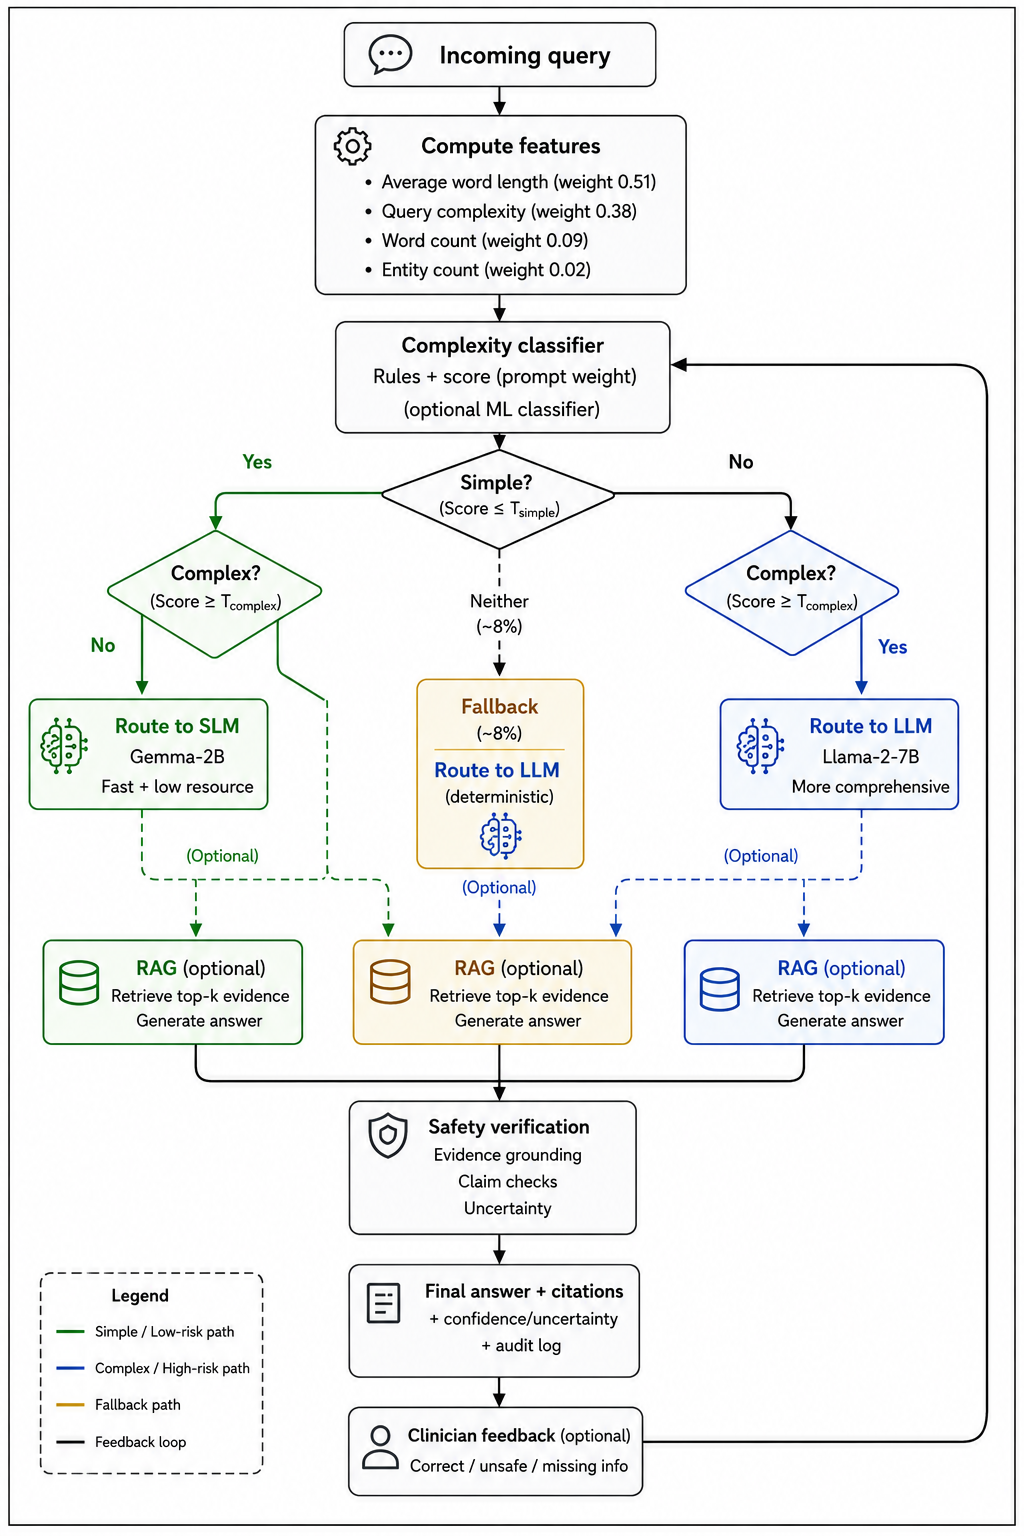
\includegraphics[width=\columnwidth]{fig_routing_decision.png}
\caption{Routing decision for assigning simple queries to the SLM and complex queries to the LLM, with optional retrieval augmentation and safety verification.}
\label{fig:routing-decision}
\end{figure}

\subsection{Phase 2: Experimental Framework and Evaluation}
\label{phase2}

A factorial $2\times2$ experimental design was used to evaluate the effect of 
retrieval augmentation across model configurations \cite{tam2024quest}. The 
core factorial analysis used three clinical queries: ``What is the treatment 
for diabetes and its associated management?'', ``How can AI assist in the 
diagnosis of disease?'', and ``What are the current guidelines for the 
management of hypertension?''. \textbf{Scope note:} this three-query set is 
an illustrative exemplar workload for demonstrating the token-F1 scoring 
protocol; it is not treated as a statistically powered quality benchmark. An extended evaluation set of 12 curated 
clinical questions spanning the six clinical domains which includes the 
three core queries was used for routing evaluation, load testing, and 
stability analysis. Each query was evaluated under two conditions: retrieval 
augmentation using the three most relevant chunks by cosine similarity, and a 
no-retrieval condition. Table~\ref{tab:query-mapping} in the Results section 
maps queries to their corresponding reported results.

The factorial design produced four experimental configurations SLM$\pm$RAG 
and LLM$\pm$RAG evaluated using the three core queries, for a total of 12 
experimental trials. This design separates model effects from retrieval 
effects and supports identification of suitable deployment configurations.

\subsubsection{Evaluation metrics and protocol}

The following evaluation measures were used. (1) \textbf{Response length 
(tokens):} an indicator of response size only, not a clinical quality metric. 
(2) \textbf{Latency:} inference time measured in seconds. (3) \textbf{RAG 
improvement (\%):} computed as $(N_{\mathrm{RAG}} - N_{\mathrm{NoRAG}}) / 
N_{\mathrm{NoRAG}} \times 100$ using token counts. (4) \textbf{Answer quality 
(F1):} the primary quality metric, computed as the harmonic mean of precision 
and recall based on token-level overlap between generated responses and 
reference answers. Reference answers were constructed for the evaluation 
dataset, and the scoring protocol is included in the reproducibility package. 
This approach follows common practice in generative question answering, where 
exact-match metrics are overly restrictive \cite{tam2024quest}. Statistical 
comparisons reported in this paper are based on F1 scores, while token-count 
improvements are reported separately as indicators of response length.

Model inference was implemented with FP16 precision, the \texttt{torch.no\_
grad()} execution context, key--value caching for token generation, and 
greedy decoding to minimize computational overhead. The combined active memory 
requirement for both models was approximately 9\,GB. Inference parameters 
were configured with a maximum of 64--128 new tokens, a minimum output length 
of 20 tokens, Greedy decoding was used for deterministic output; temperature 
and top-p parameters were set but inactive under this decoding strategy of at 
least 0.9.

\subsection{Phase 3: Retrieval-Augmented Generation with Evidence Grounding}
\label{phase3}

Throughout the factorial evaluation in this phase, \textbf{SLM}and 
\textbf{LLM}; these identifiers are used consistently throughout retrieval and generation. Post-hoc clinical-quality and faithfulness scoring 
(Table~\ref{tab:answer-quality}, Figure~\ref{fig:llm-judge-scores}) uses Qwen2.5-7B-Instruct as a separate, locally executed Hugging 
Face judge model; this judge operates independently of both the SLM and LLM 
inference pipelines and is applied only after response generation is complete.

\subsubsection{Query Routing}

Query routing is implemented as a \textbf{rule-based heuristic} , not a learned classifier. The routing logic assigns each 
incoming query to either the SLM or the LLM based on a set of deterministic 
criteria: queries are classified as \emph{simple} when they request a single 
clinical fact, definition, or direct guideline reference, and as \emph{
complex} when they involve multi-step reasoning, differential diagnosis, 
treatment comparison, or requests for synthesized evidence across multiple 
domains. Queries classified as complex are additionally flagged for retrieval 
augmentation prior to generation.

To verify implementation consistency, the heuristic was applied to a 240-query definition set (Appendix~\ref{app:routing-consistency}); held-out routing evaluation is planned for Phase~5 (Section~\ref{phase5}). Routing behavior on the Q1--Q12 workload is reported in Section~\ref{sec:routing-discussion}.

\subsubsection{Hybrid Retrieval Architecture}

This phase implements a hybrid retrieval architecture designed to improve 
response reliability through complementary retrieval mechanisms \cite{
yang2025rag, xu2025mega}. Dense retrieval captures semantic similarity 
between queries and knowledge base content using the sentence-
transformers/all-MiniLM-L6-v2 embedding model, which produces 384-
dimensional vectors indexed with FAISS IndexFlatIP. L2 normalization is 
applied to all vectors so that inner-product similarity is equivalent to 
cosine similarity, yielding an index of 556 vectors corresponding to the 
corpus segments described in Phase~1. Sparse retrieval complements the dense 
component by identifying exact clinical terminology and coding references that 
may not be well-represented in the embedding space. Results from both 
retrieval pathways are merged and re-ranked by a relevance scoring model that 
selects the top ten to fifteen documents per query. For the factorial 
evaluation, the three highest-ranked segments by cosine similarity are 
selected for context augmentation.

Retrieval latency was measured between 50 and 100\,ms per query under the 
experimental hardware configuration. This range supports near-real-time 
augmentation and is consistent with the sub-three-second end-to-end latency 
target established for the SLM deployment configuration (Section~\ref{phase1}). The hybrid strategy grounds generated responses in evidence 
retrieved from the biomedical corpus rather than relying solely on the 
parametric knowledge encoded in the language model weights, thereby reducing 
the exposure of generated outputs to factual drift or domain mismatch.

\subsubsection{Evidence Grounding and Prompt Construction}

Retrieved segments are injected into a structured prompt template prior to 
generation. The template positions the retrieved evidence before the query, 
instructing the model to confine its response to the provided context and to 
explicitly signal uncertainty when the retrieved material does not contain 
sufficient information to support a claim. This prompt structure enforces a 
soft grounding constraint at inference time and complements the claim-level 
verification mechanism applied in Phase~4 (Section~\ref{phase4}). Source 
segment identifiers are retained throughout the generation pipeline to support 
audit logging and traceability requirements described in Phase~5 
(Section~\ref{phase5}).

\subsection{Phase 4: Safety Verification and Hallucination Prevention}
\label{phase4}

A multi-stage verification process was implemented to improve the reliability 
of generated clinical responses \cite{asgari2022hallucination, 
nishizaki2025reducing}. The verification system includes an automated 
reviewer that analyzes each generated response and compares individual claims 
against the retrieved evidence, classifying each statement as supported, 
contradicted, or unsupported.

An audit logging mechanism records instances in which hallucinated statements 
are detected and blocked. These logs provide traceability for system outputs 
and support future improvements in model behavior, as well as compliance with 
regulatory and clinical validation requirements.

The safety framework operates through three verification levels aligned with 
clinical decision-support practice. The first level verifies the authenticity 
and provenance of retrieved evidence. The second level evaluates clinical 
plausibility by checking whether generated claims are consistent with the 
retrieved evidence and established medical reasoning. The third level performs 
confidence calibration, signaling uncertainty when the available evidence is 
insufficient to support a claim. As noted above, the system classifies each 
claim as supported, contradicted, or unsupported relative to the retrieved 
evidence, and claims classified as contradicted or unsupported are blocked or 
flagged before presentation to the user. Automated faithfulness scoring 
(Table~\ref{tab:answer-quality}) reports evidence-alignment rates for the RAG 
configurations; NoRAG comparability requires the extended faithfulness pass 
(\texttt{rag\_only=False}). The Phase~4 claim verifier is implemented as a 
design component, but end-to-end before/after blocking rates have not yet 
been quantitatively evaluated; these benchmarks will be reported together 
with the Phase~5 clinical validation results.

\subsection{Phase 5: Clinical Validation and Regulatory Compliance}
\label{phase5}

\textbf{Status:} Phase~5 is planned and has not yet been completed. The 
following describes the intended workflow for clinical validation and 
regulatory readiness.

This final phase is designed to evaluate the system within a clinical 
validation framework aligned with medical governance requirements \cite{
labkoff2024aicds}. A four-component evaluation framework similar to QUEST-
style assessment \cite{tam2024quest} is planned, in which licensed clinicians 
will evaluate generated responses for accuracy, clarity, and safety. Inter-
rater reliability will be measured, and the results will be documented in a 
comprehensive validation report.

\textbf{Concrete steps toward HIPAA, GDPR, and NHS-DTAC readiness} \cite{
jmir2024generative} include: (1) a Data Protection Impact Assessment (DPIA); 
(2) role-based access control mechanisms; (3) audit logging that records 
queries, retrieved segment identifiers, and system outputs without storing 
PHI; (4) PHI redaction or de-identification where applicable; (5) model risk 
management procedures, including validation and monitoring; and (6) refusal 
or uncertainty policies for unsupported or low-confidence claims. The current 
implementation already supports on-premise deployment, local processing, 
evidence-based claim verification, and audit logging; full regulatory 
validation and clinician-based evaluation will be conducted in the planned 
Phase~5 study.

\subsection{EIE Evaluation Framework}
\label{methodology:eie}

Operational resource use was assessed using the \textbf{EIE Framework} (Figure~\ref{fig:eie-framework}); measured outcomes are reported in Section~\ref{results:eie}. The framework reports NVML GPU energy and derived carbon emissions (Pillar~E), latency and VRAM observables under Context~A/B (Pillar~I), and reference electricity/hardware cost proxies (Pillar~Ec), each reported separately from clinical accuracy~\cite{ren2024reconciling, dauner2025ai, patterson2021carbon, strubell2019energy, epa2023egrid}.

\begin{figure}[!t]
\centering
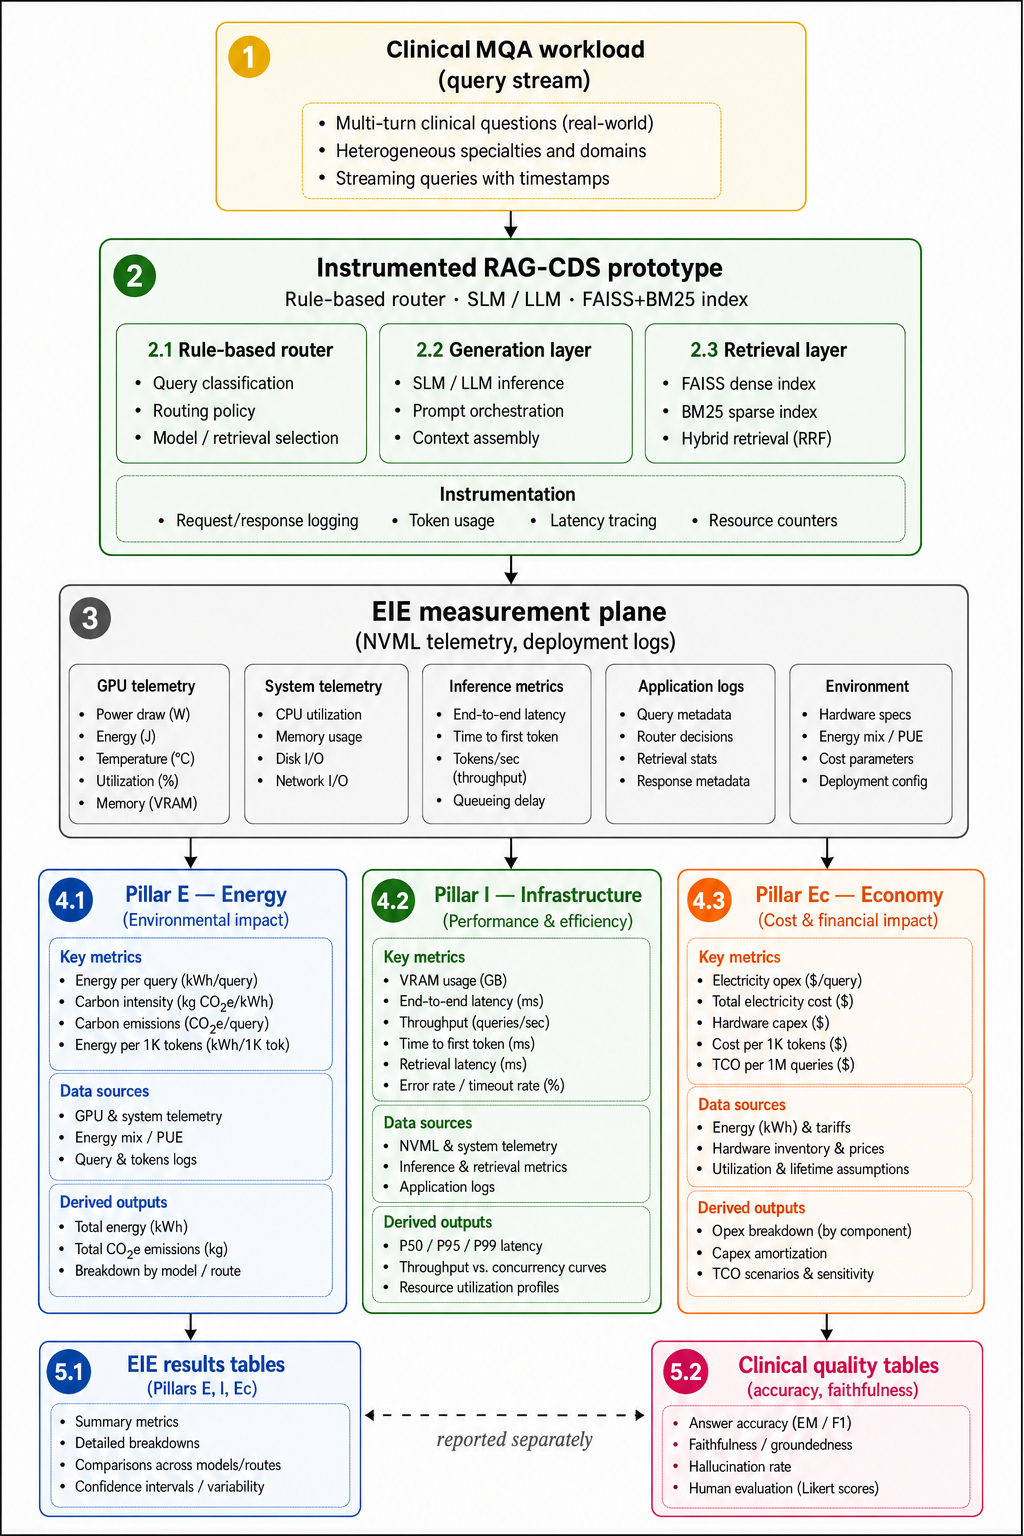
\includegraphics[width=\columnwidth]{fig_eie_framework_overview.png}
\caption{EIE framework overview for clinical MQA under RAG-CDS.}
\label{fig:eie-framework}
\end{figure}

% Include implementation section
\section{Implementation and Reproducibility}
\label{implementation-and-reproducibility}
 
\subsection{Software Infrastructure and Environment}
 
The system was implemented and evaluated using Kaggle Notebooks, a cloud-based Jupyter environment with access to NVIDIA T4 GPUs. The primary runtime environment used Python 3.9 together with established machine learning libraries. PyTorch 2.0 or later was utilized for deep learning model development, training, and inference \cite{paszke2019pytorch}. Transformers 4.30 or later facilitated model loading and inference. FAISS 1.7.4 or later enabled vector similarity search \cite{yang2025rag}. Sentence-Transformers 2.2 or later generated semantic embeddings \cite{gu2020pubmedbert}. Draft GPU sessions on Kaggle provided up to two T4 GPUs with 15 GB of memory each, 30 GB of RAM, and 57.6 GB of local disk for the energy and carbon experiments described below.
 
\subsection{Model and Library Sources}
 
Language models were sourced from the Hugging Face Model Hub. The experiments used Gemma-2-2B-it (available at as the SLM, and Llama-2-7B-chat served as the LLM \cite{amugongo2025retrieval}. Sentence-Transformers, specifically all-MiniLM-L6-v2, was employed as the embedding model. This model generates 384-dimensional semantic vectors and was selected for computational efficiency, modest memory requirements, and broad availability in resource-constrained environments. Future work will compare performance with biomedical-specific embedding models, including MedCPT, PubMedBERT, and BGE-med \cite{lee2020biobert, gu2020pubmedbert}.
 
Vector search infrastructure was implemented using FAISS (Facebook AI Similarity Search). The index utilized the IndexFlatIp configuration with inner product similarity to enable efficient similarity search and clustering \cite{yang2025rag, xiong2024rag}.
 
\subsection{Corpus Construction Pipeline}
 
Corpus construction followed established practices for biomedical knowledge base development \cite{pezoulas2023generative, zamzmi2025smd}. Semantic chunking was applied to preserve clinical context and maintain logical relationships between medical concepts \cite{alsentzer2019clinicalbert}. The final corpus contained 556 semantic chunks indexed using FAISS IndexFlatIP, with embeddings and queries L2-normalized so that inner product search corresponds to cosine similarity. Retrieval latency ranged between 50 and 100 milliseconds per query \cite{zakka2023retrieval}.
 
\subsection{Code, Data, and Reproducibility}
 
All resources used in this study are publicly available, including PubMed articles \cite{krithara2023bioasq}, clinical guidelines from FDA, NICE, and NHS \cite{labkoff2024aicds}, and Hugging Face models (Gemma-2-2B-it, Llama-2-7B-chat, and all-MiniLM-L6-v2) \cite{xiong2024rag, lee2020biobert}. Code, corpus-construction scripts, evaluation scripts, prompt templates, and aggregated evaluation logs are maintained in the project repository. The \texttt{requirements.txt} file specifies core dependencies (Python 3.9, PyTorch $\geq$2.0, Transformers $\geq$4.30, FAISS $\geq$1.7.4, Sentence-Transformers $\geq$2.2). Random seed 42 was used for numpy, torch, and CUDA where applicable. A frozen commit hash, dataset manifest, and reproduction instructions are available upon reasonable request.

Pipeline scripts cover chunking, embedding generation, index construction, inference, routing, and F1 scoring. The routing module is rule-based (not learned), using lexical features (word length, complexity, word count, entity count); implementation consistency on the 240-query definition set is reported in Appendix~\ref{app:routing-consistency}. Generation used max\_new\_tokens 64--128, temperature 0.7, top\_p $\geq$ 0.9, retrieval top-$k=3$, FP16 precision, and greedy decoding as described in Section~\ref{methodology}.

\subsection{Experimental Trial Implementation}
 
Experimental trials followed the 2$\times$2 factorial design described in \cite{tam2024quest}. The design required 12 experimental runs covering four conditions corresponding to two models and two retrieval configurations. Each condition was evaluated using three medical queries.
 
For each trial the system recorded token count, inference latency in seconds, and percentage improvement due to retrieval augmentation \cite{amugongo2025retrieval}. \textbf{Answer quality F1} was computed as the harmonic mean of precision and recall based on token level overlap between generated responses and reference answers prepared for the evaluation set. The scoring script and example annotations are included in the reproducibility package.
 
Latency and token counts were averaged across the three queries for each condition. Retrieval improvement percentages were then calculated and performance tables were generated to support comparative analysis \cite{xiong2024rag}.
 
Hallucination detection was incorporated using evidence grounded claim verification \cite{asgari2022hallucination, nishizaki2025reducing}. Generated claims were classified as supported, contradicted, or unsupported relative to retrieved evidence \cite{xu2025mega}. Energy consumption metrics were also recorded using established carbon accounting practices for AI systems \cite{ren2024reconciling, dauner2025ai}.
 
\subsection{Energy and Carbon Accounting}
 
Energy and carbon measurements were obtained using hardware-level telemetry rather than a token-based proxy. For each strategy, batches of 20 clinical queries were executed and repeated across ten independent trials on NVIDIA T4 GPUs; total GPU energy was read from NVML and normalized to kWh per query. \textbf{Scope:} reported figures are GPU-scoped only and exclude data-center overhead. Carbon emissions were derived as $E_{\mathrm{query}} \times \gamma_{\mathrm{grid}}$ with $\gamma_{\mathrm{grid}} = 0.385$\,kg CO\textsubscript{2}e/kWh~\cite{patterson2021carbon,strubell2019energy,epa2023egrid}. Results are reported in Section~\ref{results:eie}; \textbf{kWh/query} is the primary grid-independent metric~\cite{ren2024reconciling}.
 
\subsection{Privacy and Compliance}
 
The system architecture processes all queries locally and avoids transmission of data to external cloud services. This design supports alignment with HIPAA and GDPR requirements through on-premises deployment \cite{jonnagaddala2025privacy, jmir2024generative}. Queries and responses are processed locally. The audit log records system interactions, including query hashes, retrieved chunk identifiers, and verification outcomes, while avoiding storage of protected health information \cite{labkoff2024aicds, carlini2021memorization}. 
 
Concrete steps toward full HIPAA, GDPR, and NHS-DTAC readiness are described in Methodology Phase~5 (Section~\ref{phase5}). The current system provides on-premises deployment, local processing, claim verification, and audit logging; formal compliance verification remains planned.

% Include results section
\section{Results}
\label{results}

This section presents quantitative results for the SLM and LLM under RAG, NoRAG, and a hybrid routing strategy. Two \textbf{latency contexts} are used throughout and must not be conflated:
\textbf{(i) Context~A (single-query baseline)}, measured without concurrent load and used for hardware footprint and derived throughput, and
\textbf{(ii) Context~B (concurrent load)}, used for routing, load-testing, and scalability analyses.

Answer quality is evaluated primarily on open benchmarks (label accuracy on MedQA, MMLU-Med, and PubMedQA; $n{=}9{,}090$ per configuration). A supplementary three-query factorial exemplar set ($n{=}3$, Context~B) is used only to demonstrate the token-F1 scoring protocol and is not treated as primary quality evidence.

\subsection{Baseline Comparison (Context~A)}

Figure~\ref{fig:multidimensional} summarizes the SLM--LLM trade-off across six deployment dimensions. Under Context~A, the SLM achieved an inference latency of 2.3\,s, a 4\,GB model footprint, and a derived throughput of 119\,tok/s (273-token mean response length $\div$ 2.3\,s), whereas the LLM required 7.0\,s, 14\,GB, and 60\,tok/s (419 tokens $\div$ 7.0\,s). Because throughput is derived rather than independently benchmarked, it should be interpreted with care: under Context~B concurrent load (22.18\,s for the SLM and 49.55\,s for the LLM), effective per-request throughput is substantially lower.

\begin{figure}[t]
\centering
\includegraphics[width=\columnwidth]{fig_multidimensional_comparison.pdf}
\caption{Multidimensional comparison of SLM and LLM across six performance 
dimensions under Context~A baseline conditions.}
\label{fig:multidimensional}
\end{figure}

\subsection{Query Set and Mapping to Tables}

Table~\ref{tab:query-mapping} lists the curated evaluation queries and their corresponding analyses. Queries Q1--Q3 form the core 2$\times$2 factorial exemplar set used for curated-set token-F1 comparisons, while Q4--Q12 support the routing and load-testing experiments.

\begin{table}[t]
\centering
\caption{Query set and mapping to results (Q1--Q3 exemplars; Q4--Q12 extended set).}
\label{tab:query-mapping}
\footnotesize
\setlength{\tabcolsep}{3pt}
\renewcommand{\arraystretch}{1.1}

\begin{tabular}{l|p{0.46\columnwidth}|p{0.36\columnwidth}}
\hline
\textbf{ID} & \textbf{Query (abbreviated)} & \textbf{Used in} \\
\hline

Q1--Q3 & Diabetes / AI diagnosis / hypertension (factorial exemplars) & Fig.~\ref{fig:rag-scenario-responses}; Sec.~\ref{sec:routing-discussion} \\

Q4--Q12 & ACS/NSCLC/stroke/COVID-19/insulin/sepsis/HFpEF/CAR-T/anticoagulation & Routing, load test, scalability \\

\hline
\end{tabular}

\end{table}

\subsection{Corpus Statistics and Index Properties}
\label{results:corpus}

The indexed corpus comprised 115 sources yielding 556 semantic chunks (Section~\ref{phase1}). The FAISS index was approximately 100\,MB, and retrieval latency ranged from 50--100\,ms per query.

\subsection{Retrieval Performance}
\label{results:retrieval}

Retrieval quality was assessed using the hybrid dense--sparse index employed at inference (FAISS dense search with lexical BM25 re-ranking). For benchmark items with a known gold source chunk, \textbf{Recall@$k$} denotes the fraction of gold-relevant chunks found among the top-$k$ retrieved results, and \textbf{MRR} denotes the mean reciprocal rank of the first gold hit. Table~\ref{tab:retrieval-performance} reports these metrics on the \textbf{gold-label evaluable subset} $n{=}3{,}300$ per RAG configuration rows. For reference, pooling across 34 merged evaluation runs over all retrieval-attempted rows yields Recall@3 $=$ 0.919 and MRR $=$ 0.997; these supplementary figures are not used as the headline retrieval result.

\begin{table*}[htbp]
\centering
\caption{Retrieval performance on the shared hybrid index ($n{=}3{,}300$ gold-evaluable rows per RAG configuration). Both SLM+RAG and LLM+RAG use the identical FAISS+BM25 index.}
\label{tab:retrieval-performance}
\footnotesize
\setlength{\tabcolsep}{4pt}
\renewcommand{\arraystretch}{1.1}
\begin{tabular}{lccccc}
\toprule
\textbf{Configuration} &
\textbf{Recall@1} &
\textbf{Recall@3} &
\textbf{Recall@5} &
\textbf{Recall@10} &
\textbf{MRR} \\
\midrule
\textbf{RAG (both models)} & 0.667 & 0.891 & 0.914 & 0.936 & 0.967 \\

\bottomrule
\end{tabular}
\end{table*}

Strong gold-subset retrieval performance, however, did not translate uniformly into downstream accuracy gains on the open benchmarks (Table~\ref{tab:answer-quality}).

\subsection{Retrieval-Augmented Generation Effectiveness}
\label{results:rag}

RAG increased the amount of evidence-conditioned text generated by both models. Response length is reported only as a proxy for content quantity and should not be interpreted as a measure of correctness. Figure~\ref{fig:rag-scenario-responses} shows per-scenario token counts for Q1--Q3; answer quality was evaluated separately via benchmark accuracy (Table~\ref{tab:answer-quality}) and curated-set token-F1 (Section~\ref{sec:routing-discussion}).

With RAG enabled, mean response length increased from 273 to 454 tokens (+66.3\%) for the SLM and from 419 to 484 tokens (+15.5\%) for the LLM (Figure~\ref{fig:rag-scenario-responses}). Open-benchmark accuracy is reported in Table~\ref{tab:answer-quality}; curated token-F1 on three exemplar queries ($n{=}3$, Context~B) is reported in Section~\ref{sec:routing-discussion} as an illustrative methodology demonstration only and should not be conflated with open-benchmark macro-F1 or treated as a main quality conclusion.

\begin{figure}[t]
\centering
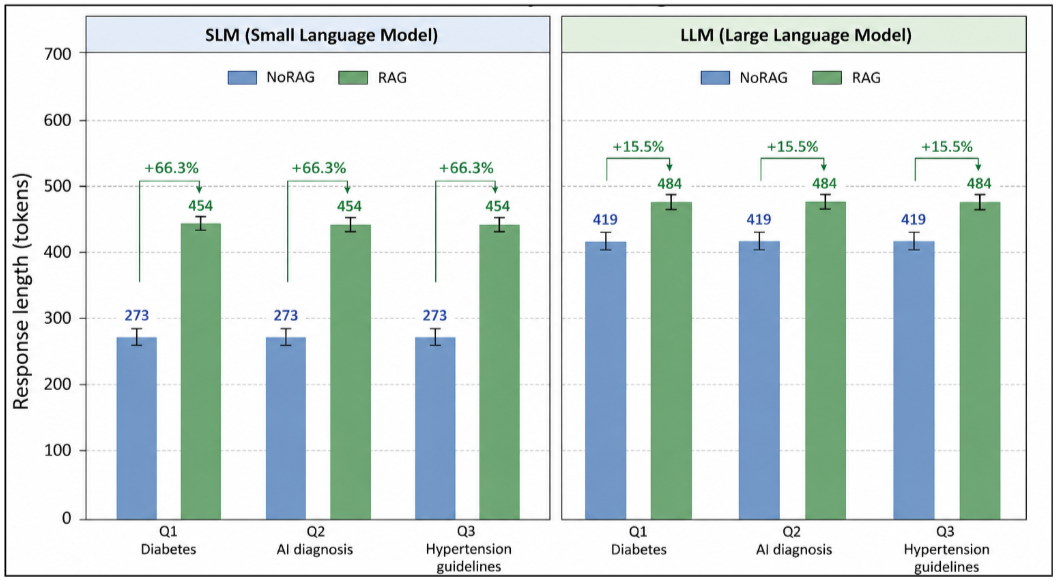
\includegraphics[width=\columnwidth]{fig_rag_scenario_responses.png}
\caption{Effect of RAG on response length (tokens) across three clinical 
scenarios for SLM and LLM.}
\label{fig:rag-scenario-responses}
\end{figure}

\subsection{Routing, Latency, and Efficiency}
\label{sec:routing-discussion}

\subsubsection{Intelligent query routing}

The routing component is a \textbf{rule-based heuristic classifier} (not a learned model) that combines four lexical features---average word length (weight 0.5141), query complexity (0.3824), word count (0.0852), and entity count (0.0183)---implemented in \texttt{eval\_routing.py}. Implementation consistency on the 240-query definition set is reported in Appendix~\ref{app:routing-consistency} and is not interpreted as held-out routing accuracy. The \textbf{primary routing evidence} is behavioral: across the 12-query extended set (Q1--Q12), 68\% of queries were routed to the SLM, 24\% to the LLM, and the remaining $\approx$8\% fell into an intermediate region handled by a deterministic fallback that defaults to the LLM.

\begin{figure}[t]
\centering
\includegraphics[width=\columnwidth]{fig_feature_importance.pdf}
\caption{Feature importance for query routing; average word length and query complexity dominate.}
\label{fig:feature-importance}
\end{figure}

\begin{table*}[htbp]
\centering
\caption{Answer quality (mean accuracy) and faithfulness (0--100, RAG rows only) by configuration ($n{=}9{,}090$ per row).}
\label{tab:answer-quality}
\footnotesize
\setlength{\tabcolsep}{4pt}
\renewcommand{\arraystretch}{1.05}
\begin{tabular}{l|c|c|c|c|c}
\toprule
\textbf{Configuration} &
\textbf{MedQA} &
\textbf{MMLU-Med} &
\textbf{PubMedQA} &
\textbf{ROUGE-L} &
\textbf{Faithfulness (\%)} \\
\midrule
SLM (No RAG) & 0.404 & 0.510 & 0.622 & 0.556 & N/A \\
SLM + RAG    & 0.403 & 0.518 & 0.596 & 0.562 & 47.2 \\
LLM (No RAG) & 0.365 & 0.421 & 0.523 & 0.328 & N/A \\
LLM + RAG    & 0.348 & 0.499 & 0.494 & 0.142 & 47.8 \\
\bottomrule
\end{tabular}
\end{table*}

\textbf{ROUGE-L drop under LLM+RAG (PubMedQA).}
The opposing ROUGE-L and token-F1 trends observed for LLM+RAG on PubMedQA warrant explanation. PubMedQA reference answers are short classification labels (``yes,'' ``no,'' or ``maybe''), which makes ROUGE-L highly sensitive to response verbosity: because RAG increases the LLM's mean response length toward 484 tokens, ROUGE-L falls (0.328$\rightarrow$0.142) relative to these terse references, even as token-F1 computed against the retrieved-chunk vocabulary rises (0.049$\rightarrow$0.172). SLM ROUGE-L, by contrast, remains stable (0.556$\rightarrow$0.562). \textbf{Label accuracy} in Table~\ref{tab:answer-quality} remains the primary PubMedQA metric; ROUGE-L is reported for completeness only.

\subsubsection{Benchmark error analysis}
\label{results:error-analysis}

Table~\ref{tab:answer-quality} shows that RAG did not uniformly improve label accuracy. Three factors help explain these mixed outcomes.

\textbf{Corpus--benchmark mismatch (MedQA).}
MedQA items often require reasoning over USMLE-style clinical vignettes whose topical coverage is broader than our 115-document corpus (112 PubMed articles and three guidelines). When retrieved segments are only weakly related to the vignette, RAG can inject off-topic context that competes with parametric knowledge. This plausibly explains the small MedQA decreases under RAG (SLM: 0.404$\rightarrow$0.403; LLM: 0.365$\rightarrow$0.348) despite strong gold-subset retrieval metrics (Recall@3 $=0.891$).

\textbf{Response-format mismatch (PubMedQA).}
PubMedQA is scored by short yes/no/maybe labels, whereas RAG prompts encourage longer evidence-grounded explanations. The LLM+RAG configuration therefore shows lower PubMedQA label accuracy (0.523$\rightarrow$0.494) alongside increased verbosity, consistent with format mismatch rather than uniformly worse medical content.

\textbf{Model--task interaction (LLM vs.\ SLM).}
On the open benchmarks, Gemma-2-2B-it (SLM) outperformed Llama-2-7B-chat (LLM) on MedQA and PubMedQA in both NoRAG and RAG settings. This may reflect instruction-tuning differences, decoding behavior, or benchmark-format sensitivity rather than a general claim that smaller models are clinically superior. The primary conclusion supported by $n{=}9{,}090$ predictions per configuration is that RAG effects are \emph{task dependent}, not uniformly beneficial.

\textbf{Partial faithfulness ($\approx$47--48\%).}
Automated faithfulness scores near 50\% indicate that roughly half of judged answer content received only partial or indirect support from retrieved passages under the Qwen2.5-7B-Instruct rubric (40--55 partial-support band). This is consistent with retrieval noise, multi-claim answers in which only some sentences are grounded, and strict judge criteria. It motivates corpus expansion, reranking refinement, and quantitative Phase~4 claim-verifier blocking rates in future work.

\begin{figure}[t]
\centering
\includegraphics[width=\columnwidth]{fig_routing_decisions.pdf}
\caption{Routing confidence vs.\ latency per query on the Q1--Q12 workload set.}
\label{fig:routing-decisions}
\end{figure}

\subsubsection{Static and routing comparison under load}

Under Context~B concurrent load on Q1--Q12, the SLM-only, LLM-only, and hybrid-routing strategies occupy distinct positions on the latency frontier. A supplementary three-query token-F1 exemplar ($n{=}3$) is reported only in the limitations (Section~\ref{discussion}) to demonstrate the scoring protocol and is not used as primary quality evidence.

\subsection{Clinical Answer Quality (LLM-as-Judge)}
\label{results:llm-judge}

Model-based clinical scoring complements the overlap-based metrics. Qwen/Qwen2.5-7B-Instruct rated each response on a 0--5 rubric for \emph{correctness}, \emph{completeness}, and \emph{clinical relevance}. Figure~\ref{fig:llm-judge-scores} reports mean scores on the judged subset ($n{=}8{,}950$ for SLM+RAG and $n{=}8{,}965$ for all other configurations). Coverage was 35,845 of 36,360 predictions (98.6\%), with 515 rows left unjudged (140 for SLM\_RAG and 125 for each remaining configuration).

\begin{figure}[t]
\centering
\includegraphics[width=\columnwidth]{fig_llm_judge_scores.pdf}
\caption{LLM-as-judge clinical scores (Qwen2.5-7B-Instruct; 0--5 scale). RAG vs.\ NoRAG differences are negligible in effect size.}
\label{fig:llm-judge-scores}
\end{figure}

RAG-versus-NoRAG judge-score differences were small ($|\Delta| \leq 0.13$; Cohen's $d < 0.15$). These scores reflect within-run rankings rather than evidence of clinical approval.

\subsection{Scalability and System Stability}

Latency increased non-linearly with user load: scaling from 5 to 10 concurrent users increased latency by approximately 2.24$\times$. All configurations maintained stable token generation without truncation. Peak GPU memory under concurrent load is reported in Table~\ref{tab:eie-infrastructure}.


\subsection{EIE Framework Assessment}
\label{results:eie}

Deployability was assessed using the \textbf{EIE (Energy--Infrastructure--Economy) Framework} defined in Section~\ref{methodology:eie} (Figure~\ref{fig:eie-framework}). GPU energy was measured via NVML telemetry across 10 trials $\times$ 20 clinical queries per strategy~\cite{patterson2021carbon,strubell2019energy}. \textbf{Scope:} all Pillar~E measurements are GPU-scoped only and exclude data-center overhead. Carbon emissions were derived from measured kWh using $\gamma_{\mathrm{grid}} = 0.385$\,kg CO\textsubscript{2}e/kWh~\cite{epa2023egrid}; \textbf{kWh/query} remains the primary, grid-independent metric. Pillar observables are reported separately from clinical accuracy and faithfulness (Table~\ref{tab:answer-quality}).

\subsubsection{Pillar E: Energy and carbon emissions}

Table~\ref{tab:energy-carbon} reports per-query GPU energy (mean$\,\pm$\,std) and derived CO\textsubscript{2}e for all five strategies. Figure~\ref{fig:eie-energy-carbon} visualizes the same Pillar~E observables: per-query energy intensity (bars) and derived CO\textsubscript{2}e per million queries (line). RAG added negligible mean energy ($<$2\%) relative to NoRAG within each model class, and pairwise kWh ratios are invariant to grid carbon intensity~\cite{ren2024reconciling}.

\begin{table}[htbp]
\centering
\caption{Pillar~E: per-query GPU energy and derived carbon (NVML; $\gamma_{\mathrm{grid}} = 0.385$\,kg/kWh; GPU-scoped, excludes data-center overhead).$^{*}$}
\label{tab:energy-carbon}
\footnotesize
\setlength{\tabcolsep}{4pt}
\renewcommand{\arraystretch}{1.12}
\begin{tabular}{l|c|c}
\toprule
\textbf{Strategy} & \textbf{kWh/query} & \textbf{CO\textsubscript{2}e/M (kg)} \\
\midrule
SLM\_NoRAG      & 0.000052 $\pm$ 0.000011 & 19.83 \\
SLM\_RAG        & 0.000052 $\pm$ 0.000013 & 19.82 \\
LLM\_NoRAG      & 0.000111 $\pm$ 0.000024 & 42.35 \\
LLM\_RAG        & 0.000112 $\pm$ 0.000023 & 42.47 \\
Routing\_Hybrid & 0.000101 $\pm$ 0.000021 & 38.19 \\
\bottomrule
\end{tabular}

\vspace{2pt}
\noindent\footnotesize $^{*}$CO\textsubscript{2}e/M from full-precision kWh means; displayed kWh rounded ($\leq$1.8\% mismatch). GPU scope only.
\end{table}

\begin{figure}[htbp]
\centering
\includegraphics[width=\columnwidth]{fig_eie_energy_carbon.pdf}
\caption{Pillar~E: per-query energy intensity (kWh/query) and derived CO\textsubscript{2}e per million queries across deployment strategies. SLM\_RAG consumed approximately 2.15$\times$ less energy per query than LLM\_RAG.}
\label{fig:eie-energy-carbon}
\end{figure}

\subsubsection{Pillar I: Infrastructure}

Table~\ref{tab:eie-infrastructure} summarizes the Pillar~I observables.

\begin{table}[htbp]
\centering
\caption{Pillar~I: infrastructure observables (SLM+RAG vs.\ LLM+RAG).}
\label{tab:eie-infrastructure}
\footnotesize
\setlength{\tabcolsep}{4pt}
\renewcommand{\arraystretch}{1.1}
\begin{tabular}{l|c|c|c}
\toprule
\textbf{Metric} & \textbf{SLM+RAG} & \textbf{LLM+RAG} & \textbf{Ratio} \\
\midrule
VRAM footprint (GB) & 4 & 14 & 3.50$\times$ \\
Latency Context~A (s) & 2.3 & 7.0 & 3.04$\times$ \\
Latency Context~B (s) & 22.18 & 49.55 & 2.23$\times$ \\
Throughput (tok/s) & 119 & 60 & 1.98$\times$ \\
Peak GPU load (GB) & \multicolumn{2}{c|}{14.28--14.37} & N/A \\
\bottomrule
\end{tabular}

\vspace{2pt}
\noindent\footnotesize $^{\ddagger}$Derived from Context~A only.
\end{table}

\subsubsection{Pillar Ec: Economy (electricity and hardware cost)}

Electricity operating expense was computed from measured kWh using a reference U.S.\ tariff of \$0.12/kWh, and hardware amortization assumes reference GPU capex tiers depreciated over three years. Table~\ref{tab:eie-economy} summarizes the annual electricity and amortized hardware costs by strategy.

\begin{table}[htbp]
\centering
\caption{Pillar~Ec: annual electricity and amortized hardware cost (USD reference tariffs).}
\label{tab:eie-economy}
\footnotesize
\setlength{\tabcolsep}{3pt}
\renewcommand{\arraystretch}{1.1}
\begin{tabular}{l|c|c|c}
\toprule
\textbf{Strategy} & \textbf{Elec./yr} & \textbf{GPU amort./yr} & \textbf{Combined/yr} \\
\midrule
SLM\_RAG & \$2{,}278 & \$117 & \$2{,}395 \\
LLM\_RAG & \$4{,}901 & \$400 & \$5{,}301 \\
Routing\_Hybrid & \$4{,}422 & \$400 & \$4{,}822 \\
\bottomrule
\end{tabular}

\vspace{2pt}
\noindent\footnotesize Elec./yr = measured kWh $\times$ \$0.12; hardware amort.\ = reference capex $\div$ 3 yr.
\end{table}

% Include discussion section
\section{Discussion}
\label{discussion}

This section interprets the results (Section~\ref{results}) in relation to the three research questions, discusses implications for deployment, and outlines study limitations.

\subsection{Addressing Research Question 1: Efficiency Quality Trade off}

\textbf{Open benchmarks as primary quality evidence.}
On the open benchmarks (Table~\ref{tab:answer-quality}, $n{=}9{,}090$ per configuration), RAG effects were mixed: MMLU-Med improved for the LLM (+18.5\%; 0.421$\rightarrow$0.499), whereas PubMedQA label accuracy decreased for both models ($-$4.2\% SLM, $-$5.5\% LLM). Section~\ref{results:error-analysis} analyzes plausible causes, including corpus--benchmark mismatch and response-format effects. A supplementary three-query token F1 exemplar ($n{=}3$) is reported only in the limitations below and must not be interpreted as primary quality evidence.

\textbf{Infrastructure and energy.}
Under Context~A and Context~B, the SLM required substantially less VRAM, lower single-query latency, and lower NVML-measured energy than the LLM (Tables~\ref{tab:eie-infrastructure} and~\ref{tab:energy-carbon}). RAG added less than 2\% mean GPU energy relative to NoRAG within each model class.

RQ1 is therefore \textbf{partially answered}: SLM+RAG demonstrates lower measured resource use on T4 GPUs with comparable automated faithfulness scores; however, open benchmark quality gains are inconsistent, and the three query token-F1 result is illustrative only.

\subsection{Addressing Research Question 2: Hallucination Prevention}

Automated faithfulness scores (Table~\ref{tab:answer-quality}) average 47.2\% for SLM+RAG and 47.8\% for LLM+RAG, both within the partial support rubric band (40--55). Because NoRAG faithfulness scoring was not completed, a quantitative RAG-vs.-NoRAG grounding comparison is \textbf{not reported}. LLM as judge RAG vs.NoRAG deltas were negligible in effect size (Figure~\ref{fig:llm-judge-scores}).

The Phase~4 claim verifier (supported/contradicted \\ /unsupported) is implemented as a design component, but end-to-end blocking rates were not measured. RQ2 is therefore \textbf{partially answered}, addressing only the absolute RAG faithfulness levels. Broader safety conclusions require NoRAG baselines, claim verifier benchmarks, and Phase~5 clinician review.

\subsection{Addressing Research Question 3: Privacy, Sustainability, and Compliance}

The system processes queries locally without cloud APIs; audit logging and PHI-minimizing design are intended to support HIPAA/GDPR \emph{readiness}, though formal compliance is not certified and no real-world clinical safety or effectiveness results are presented. EIE reporting keeps these operational metrics separate from the clinical results tables (Section~\ref{results:eie}).

\textbf{Routing.}
The router is rule based. Perfect agreement on the 240 query definition set is reported only as an \textbf{implementation consistency check} (Appendix~\ref{app:routing-consistency}), not as routing accuracy or held-out validation. The primary behavioral evidence is provided by the Q1--Q12 split (68\% routed to the SLM, 24\% to the LLM, and $\approx$8\% to a fallback defaulting to the LLM), along with end to end latency under concurrent load.

GPU memory under concurrent load remained stable, with a peak of 14.28--14.37\,GB (Table~\ref{tab:eie-infrastructure}). Scaling from 5 to 10 users increased latency by approximately 2.24$\times$.

\subsection{Implications for Clinical AI Deployment}

These results indicate that resource-constrained sites may consider SLM+RAG deployments due to their 4\,GB footprint and lower NVML measured energy use, while privacy sensitive institutions may benefit from on premise processing. For sustainability reporting, measured kWh should serve as the primary, grid independent metric, with derived carbon figures reported alongside the stated $\gamma_{\mathrm{grid}}$ value. Regulatory deployment pathways still require Phase~5 clinician validation. Automated scores alone do not constitute clinical approval, and this manuscript does not claim safety for validated bedside deployment.

\subsection{Comparison with Prior Work}

This study contributes SLM--LLM comparisons under hybrid retrieval, NVML-based energy measurement, and an explicit EIE decomposition, alongside a mixed pattern of open-benchmark outcomes. Prior RAG work has often emphasized accuracy alone, without joint infrastructure and cost reporting~\cite{yang2025rag,ren2024reconciling}.

\subsection{Retrieval-Augmented Generation: Common Failure Modes and Mitigations}

Strong gold-subset retrieval performance (Recall@3 $=0.891$, MRR $=0.967$) did not consistently translate into improved downstream benchmark accuracy. This outcome is consistent with retrieval noise and task format effects, such as the mismatch between PubMedQA's terse label accuracy and the models' more verbose generations. Potential mitigations include curated corpora, hybrid retrieval, faithfulness scoring, and the planned claim verification pipeline.

\subsection{Limitations and Future Work}

\textbf{Two evaluation contexts for F1 and accuracy.} The distinction between the curated set ($n{=}3$) and the open benchmarks ($n{=}9{,}090$) must remain explicit throughout, as the two are not directly comparable. The three query token-F1 experiment (SLM+RAG 0.6101 vs.\ LLM+RAG 0.4548 vs.\ hybrid 0.5667 under Context~B) is illustrative only and should not support strong quality conclusions; readers should note the $n{=}3$ warning if token F1 is displayed.

\textbf{Clinical validation.} Clinical validation by practicing physicians (Phase~5) is planned as follow up work; this manuscript does not present real world clinical safety or effectiveness results.

\textbf{Automated judges.} Qwen2.5-7B-Instruct is used to score faithfulness and clinical quality; these scores serve as within-run proxies and do not constitute clinician validation.

\textbf{Faithfulness and Phase~4.} NoRAG faithfulness evaluation remains pending, and claim-verifier blocking rates have not yet been quantified.

\textbf{Routing generalization.} Held out routing evaluation and learned routers fall outside the scope of the current rule-based design.

\textbf{Corpus scope.} The corpus of 115 documents and 556 chunks spans six clinical domains but does not cover the full breadth of clinical medicine.

Future work will include Phase~5 clinician review, completion of the NoRAG faithfulness evaluation, expanded benchmark coverage, corpus updates, and prospective deployment studies.

% Include conclusion section
\section{Conclusion}
\label{conclusion}
We evaluated SLM and LLM configurations under NoRAG, RAG, and rule based hybrid routing for medical question answering on a 115 document biomedical corpus and open MQA benchmarks ($n{=}9{,}090$ predictions per configuration). Within this evaluated corpus, model, and benchmark scope, on NVIDIA T4 GPUs, SLM\_RAG consumed approximately 2.15$\times$ less energy per query and produced approximately 2.14$\times$ lower CO\textsubscript{2}e/M than LLM\_RAG, with comparable automated faithfulness scores ($\approx$47--48\%) and strong retrieval metrics on the gold evaluable subset (Recall@3 $=0.891$, MRR $=0.967$). Open-benchmark RAG effects were mixed (Table~\ref{tab:answer-quality}), indicating that retrieval gains do not uniformly transfer to downstream label accuracy; Section~\ref{results:error-analysis} discusses plausible failure modes. Routing implementation consistency on a rule-constructed definition set is reported in Appendix~\ref{app:routing-consistency} and is not interpreted as held out predictive accuracy. NoRAG faithfulness baselines and quantitative claim verifier blocking rates remain directions for future work, as does expanded curated evaluation (50--100+ questions with formal statistics). Clinical validation by practicing physicians (Phase~5) and formal regulatory assessment are planned as next steps; this manuscript does not present real world clinical safety or effectiveness results.


% Include appendix
\appendices
\section{Routing Implementation Consistency Check}
\label{app:routing-consistency}

Query routing is implemented using a rule-based heuristic instead of a learned classifier. To verify alignment between implementation and specification, the heuristic was applied to a definition set of 240 queries. This set was constructed by expanding 12 core evaluation queries into 20 lexical and syntactic paraphrases each. Labels for this set were generated using the same rule criteria as the heuristic, ensuring that the label generation process and the classifier remain definitionally aligned.

On this definition set, classifier outputs matched the rule-generated labels on all 240 queries. We report this as an \textbf{implementation consistency check}, not as routing accuracy or held-out predictive performance. The primary routing evidence in the main text is behavioral: the Q1--Q12 workload split (68\% routed to the SLM, 24\% to the LLM, and $\approx$8\% to a fallback defaulting to the LLM) together with end-to-end latency under concurrent load (Section~\ref{sec:routing-discussion}).

Evaluation of routing on held-out queries from sources external to the definition set is scheduled for Phase~5 clinical validation (Section~\ref{phase5}).


\vspace{1em}
\textit{Disclosure:} The authors used AI tools, including Perplexity Pro, Cursor Pro, Hugginface Pro, and other AI-assisted tools during the preparation of this manuscript.

% Include references
\input{references}

\EOD
\end{document}
